\subsection{Machine Learning Models Used in This Project}
\begin{enumerate}
	\item \textbf{K-nearest Neighbors}
	The K-Nearest Neighbors (K-NN) algorithm is one of the simplest machine learning algorithms, based on the supervised learning technique. It assumes similarity between the new case/data and available cases, categorizing the new case into the most similar available category. K-NN stores all available data and classifies new data points based on similarity, making it a convenient method for classifying new data into suitable categories.
	
	K-NN can be used for both regression and classification, though it is primarily used for classification problems. It is a non-parametric algorithm, meaning it does not make any assumptions about the underlying data distribution. Also known as a lazy learner algorithm, K-NN does not immediately learn from the training set but rather stores the dataset and performs actions upon classification.
	
	For example, consider two categories, Category A and Category B. If we have a new data point x1, K-NN helps determine whether this data point belongs to Category A or B. The process can be visualized in the diagram below:
	\begin{figure}[h]
		\centering
		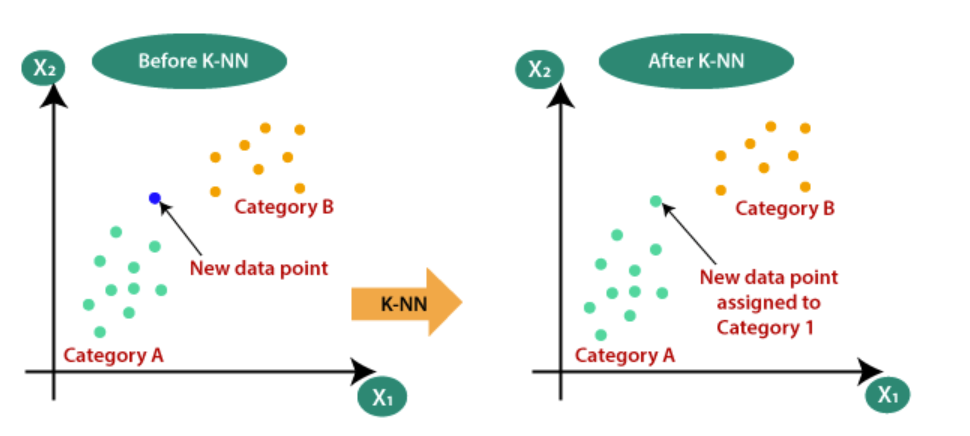
\includegraphics[width=1\textwidth]{picture/KNN1}
		\caption{Illustration of K-NN Classification}
		\label{fig:knn1}
	\end{figure}
	
	\textbf{How Does K-NN Work?}
	The K-NN algorithm operates as follows:
	
	\begin{enumerate}
		\item Select the number K of neighbors.
		\item Calculate the Euclidean distance of K neighbors.
		\item Take the K nearest neighbors as per the Euclidean distance.
		\item Count the number of data points in each category among these K neighbors.
		\item Assign the new data points to the category with the maximum number of neighbors.
		\item The model is ready.
	\end{enumerate}
	Suppose we have a new data point that needs categorization. First, we choose the number of neighbors (k=5). Next, we calculate the Euclidean distance between the data points, as shown below:
	\begin{figure}[h]
		\centering
		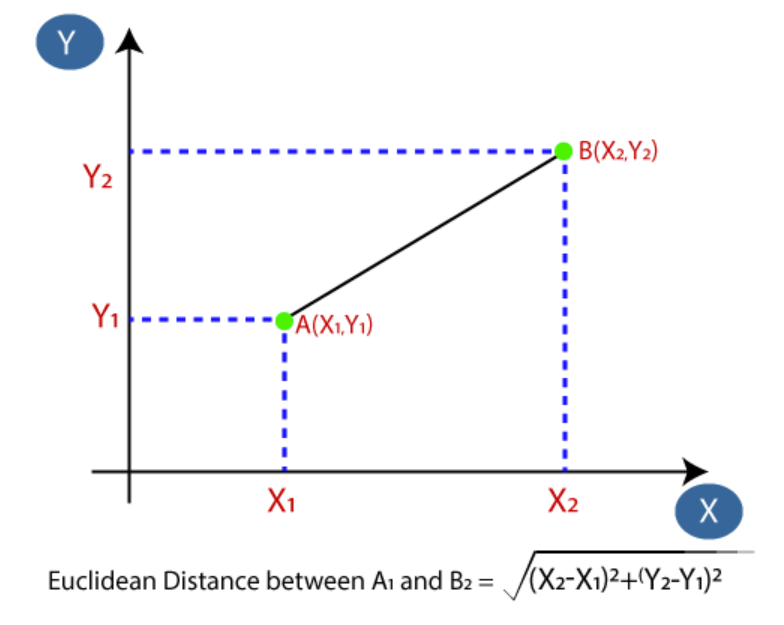
\includegraphics[width=0.5\textwidth]{picture/KNN2}
		\caption{Euclidean Distance Calculation in K-NN}
		\label{fig:knn2}
	\end{figure}
	
	After calculating the Euclidean distance, we identify the nearest neighbors. For instance, if there are three nearest neighbors in Category A and two in Category B, as illustrated in the image below, the new data point would most likely belong to Category A.
	\begin{figure}[h]
		\centering
		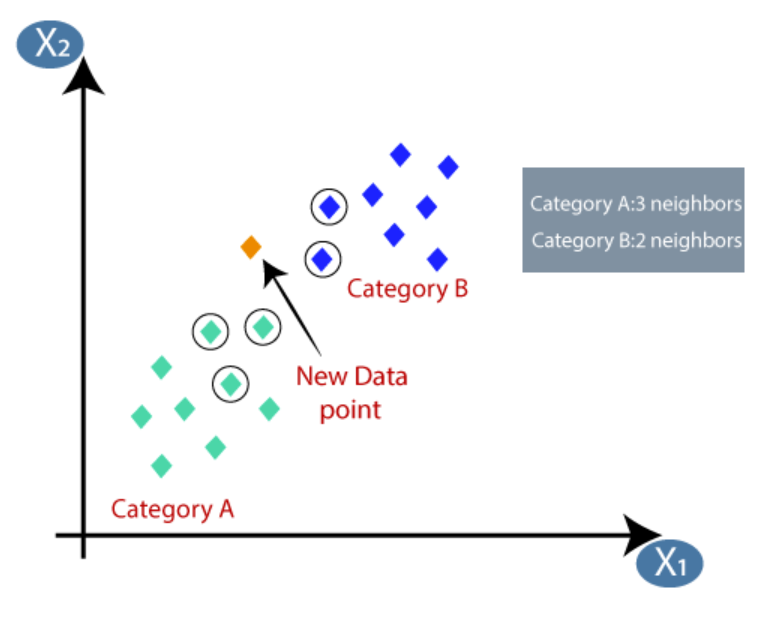
\includegraphics[width=0.5\textwidth]{picture/KNN3}
		\caption{Identifying Nearest Neighbors in K-NN}
		\label{fig:knn3}
	\end{figure}
	
\item \textbf{Random Forest}
Random Forest is a supervised learning algorithm known for its versatility. It constructs a “forest” which is an ensemble of decision trees, typically trained using the bagging method. This method involves combining multiple learning models to improve the overall result.

Random Forest is effective because it constructs multiple decision trees and merges them to achieve a more accurate and stable prediction. This algorithm is advantageous as it can be applied to both classification and regression problems, which are prevalent in many machine learning systems.

\textbf{Random Forest in Classification and Regression}
In classification, which is often considered a fundamental aspect of machine learning, Random Forest operates effectively. The following figure illustrates a Random Forest model with two trees:
\begin{figure}[h]
	\centering
	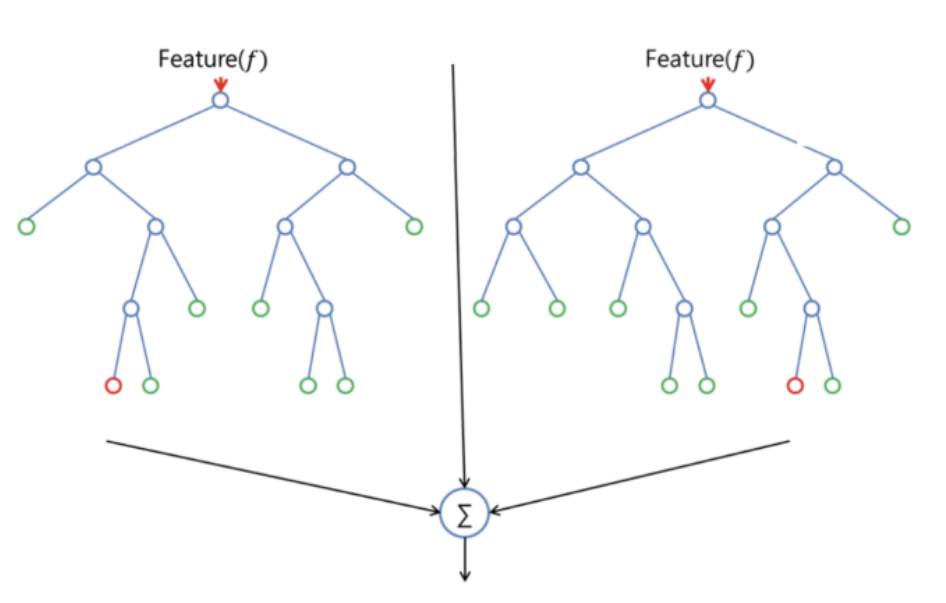
\includegraphics[width=0.5\textwidth]{picture/RF1}
	\caption{Example of a Random Forest Model with Two Trees}
	\label{fig:random_forest}
\end{figure}

Random Forest shares many hyperparameters with decision trees and bagging classifiers. It simplifies the process by combining these elements into a single classifier. The classifier can be adjusted to handle regression tasks as well, using the regressor class of Random Forest.

The algorithm introduces additional randomness into the model during tree construction. Instead of searching for the most important feature while splitting a node, it searches among a random subset of features. This approach enhances diversity and typically yields a better model.

In a Random Forest classifier, only a random subset of features is considered for splitting a node. Trees can be made even more random by using random thresholds for each feature rather than the best possible thresholds, as is done in standard decision trees.

\textbf{Random Forest Models vs. Decision Trees}
Random Forest, while a collection of decision trees, differs significantly in its approach. A decision tree creates a set of rules from a training dataset, which it then uses to make predictions. For example, in predicting online advertisement clicks, a decision tree will generate rules based on past click data and associated features.

In contrast, Random Forest selects random observations and features to construct several decision trees and then averages their predictions. This method helps mitigate overfitting, which is a common issue with “deep” decision trees. Random Forest achieves this by creating random subsets of features, building smaller trees, and then combining them. However, it’s important to note that this approach may increase computational time and doesn't always prevent overfitting, depending on the number of trees constructed.

	\item \textbf{Logistic Regression}
\end{enumerate}

\subsection{Confusion Matrix}
A confusion matrix is a table typically used to describe the performance of a classification model on a set of test data for which the true values are known. It visualizes the model's accuracy by comparing the actual target values with the predictions made by the machine learning model.

Consider the following example of a confusion matrix:
\begin{figure}[h]
	\centering
	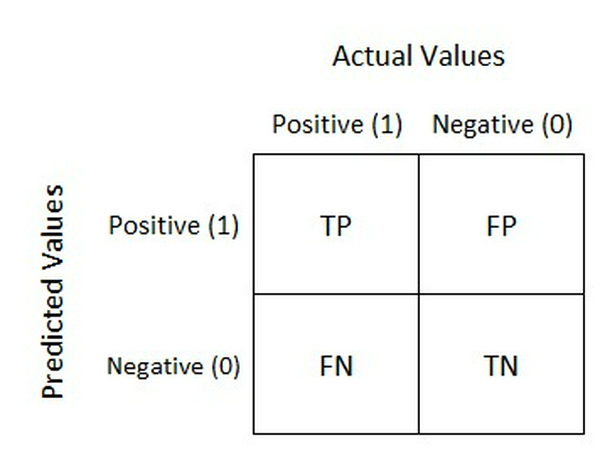
\includegraphics[width=0.5\textwidth]{picture/confusion}
	\caption{Confusion Matrix Example}
	\label{fig:confusion_matrix}
\end{figure}

The key components of a confusion matrix are:
\begin{itemize}
	\item \textbf{True Positive (TP)}: Instances where the model correctly predicts the positive class.
	\item \textbf{True Negative (TN)}: Instances where the model correctly predicts the negative class.
	\item \textbf{False Positive (FP)}: Instances where the model incorrectly predicts the positive class, also known as a Type I error.
	\item \textbf{False Negative (FN)}: Instances where the model incorrectly predicts the negative class, also known as a Type II error.
\end{itemize}

In the case of a multi-class classification problem, such as the Iris dataset, the confusion matrix will have dimensions of \( n\_classes \times n\_classes \). Each entry (i, j) in the matrix corresponds to the number of instances where class i was predicted as class j.

\subsection{Classification Report}
The classification report presents several key metrics for each class, which are essential for evaluating the performance of a classification model:

\begin{itemize}
	\item \textbf{Precision}: This metric is the ratio of correctly predicted positive observations to the total predicted positives. It addresses the question, "Of all instances labeled as positive by the model, how many are actually positive?" Precision is calculated as TP / (TP + FP), where TP is the number of true positives and FP is the number of false positives.
	
	\item \textbf{Recall} (also known as Sensitivity or True Positive Rate): Recall is the ratio of correctly predicted positive observations to all observations in the actual class. It answers the question, "Of all the instances that are actually positive, how many were correctly labeled by the model?" It is calculated as TP / (TP + FN), where FN is the number of false negatives.
	
	\item \textbf{F1-Score}: This score is the weighted harmonic mean of precision and recall. It considers both false positives and false negatives, making it a robust measure that shows the balance between precision and recall. The F1-Score is calculated as 2 * (Precision * Recall) / (Precision + Recall).
	
	\item \textbf{Support}: This indicates the number of actual occurrences of each class in the specified dataset. For instance, if Iris-setosa has a support of 11, it means there are 11 instances of Iris-setosa in the test set that the model has attempted to predict.
	
	\item \textbf{Accuracy}: Accuracy represents the ratio of correctly predicted observations to the total observations. It is expressed as (TP + TN) / Total, where TN is the number of true negatives.
	
	\item \textbf{Macro Average}: This is the average of precision, recall, and F1-score calculated between classes, without considering class imbalance. It gives equal weight to each class.
	
	\item \textbf{Weighted Average}: In contrast to the macro average, the weighted average of precision, recall, and F1-score is calculated between classes while taking into account the number of instances in each class. This approach weights each class proportionally to its presence in the dataset.
\end{itemize}
